\section{Visualisierung des Algorithmus} \label{chap:Visualisierung}


Ein Seiten-Tab-Reiter des R-Shiny-Dashboards, wird der Visualisierung des Algorithmus gewidmet. 
Dieser besteht aus drei Unter-Reitern, in denen Generationen von Ameisen visuell gezeigt werden und der Algorithmus auf die Rosenbrock- und auf die Himmelblaufunktion angewendet wird. Den zugehörigen Quellcode-Ausschnitt der app\_ui.R Datei zeigt Abbildung \ref{fig:app_ui_visualisations_tab}. 

\begin{figure}[H]
 \centering
 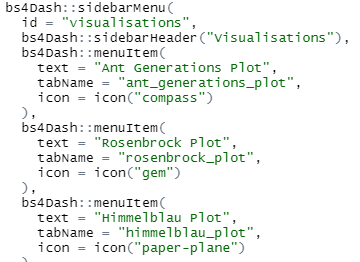
\includegraphics[scale=1]{"images/04_Visualisierung_des_Algorithmus/app_ui_visualisations_tab.png"}
 \caption{Quellcode in app\_ui.R zur Darstellung des seitlichen Navigation-Tab-Reiters für Visualisierungen des ACO}
 \label{fig:app_ui_visualisations_tab}
\end{figure}

In den beiden Unter-Reitern \textit{Rosenbrock Plot} und \textit{Himmelblau Plot} werden die Optimierungsfunktionen jeweils in einem 3d-Plot dargestellt. Die Funktion, die diesen Graph generiert, zeigt Abbildung \ref{fig:util_3dplot}.
Dem Benutzer werden hierbei interaktive Schieberegler zur Veränderung der Darstellung des Plots in der rechten Seitenleiste zur Verfügung gestellt. Diese werden in Abbildung \ref{fig:ui_RoseHimPlot_2} dargestellt. 

\begin{figure}[H]
 \centering
 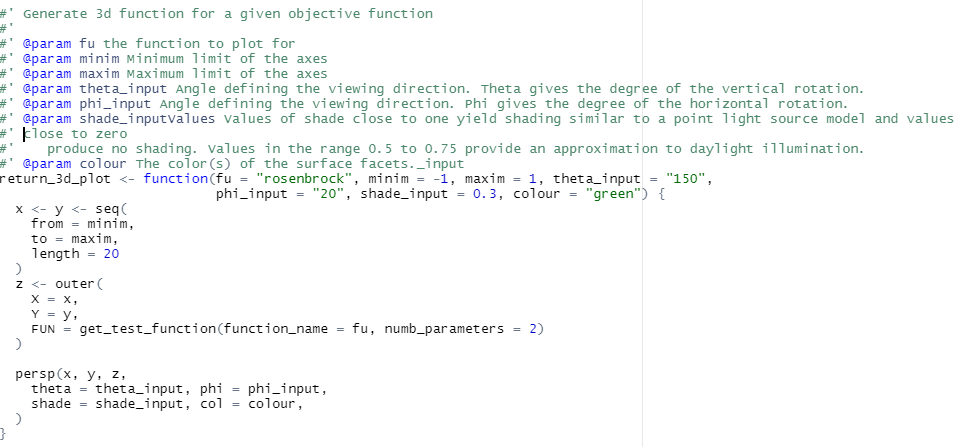
\includegraphics[scale=0.7]{"images/04_Visualisierung_des_Algorithmus/util_3dplot.png"}
 \caption{Funktion in global\_utils.R zur Generierung eines dreidimensionalen Graphen der Rosenbrock- oder Himmelblau-Funktion)}
 \label{fig:util_3dplot}
\end{figure}


\begin{figure}[H]
 \centering
 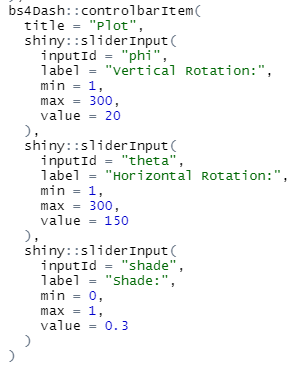
\includegraphics[scale=.7]{"images/04_Visualisierung_des_Algorithmus/ui_slider_for_rose_him_plots_2.png"}
 \caption{Quellcode in fct\_update\_controlbar.R zur Darstellung interaktiver Elemente für die Ansicht und Schattierung des drei-dimensionalen Graphen der Optimierungsfunktion (Rosenbrock oder Himmelblau-Funktion)}
 \label{fig:ui_RoseHimPlot_2}
\end{figure}

Weiterhin wird das tatsächliche Minimum der Rosenbrockfunktion in global\_utils.R, der Datei für globale Funktionen, berechnet und in Form eines Data-Frames gespeichert, um sie auf dem Dashboard in Form einer Tabelle darstellen zu können (siehe Abbildung \ref{fig:global_Mimima_Rose}). Die Minima der Himmelblau-Funktion werden ebenfalls in Form eines Data Frames gespeichert (siehe Abbildung \ref{fig:global_Mimima_Him}). Hierbei wird nur eines der Minima berechnet, während die weiteren drei Minima werden manuell hinzugefügt werden. 

\begin{figure}[H]
 \centering
 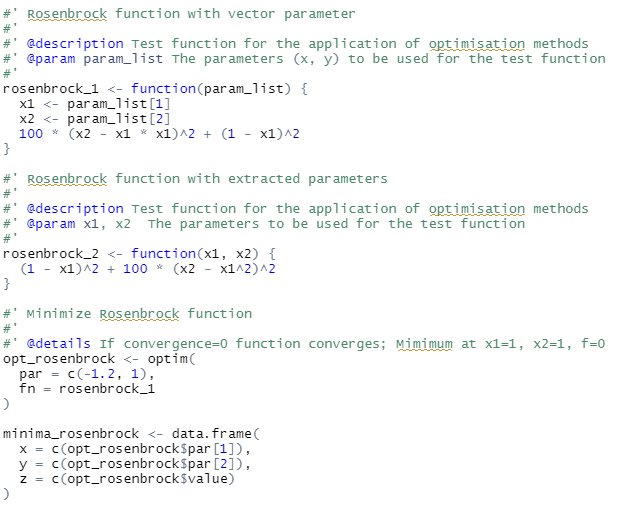
\includegraphics[scale=.7]{"images/04_Visualisierung_des_Algorithmus/utilsR_Minima_Rosenbrock.png"}
 \caption{Quellcode in global\_utils.R zur Erfassung und Speicherung des tasächlichen Minimums der Rosenbrock-Funktion}
 \label{fig:global_Mimima_Rose}
\end{figure}

\begin{figure}[H]
 \centering
 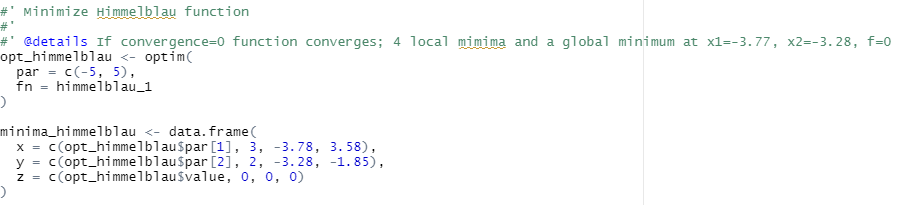
\includegraphics[scale=0.7]{"images/04_Visualisierung_des_Algorithmus/utilsR_Minima_Himmelblau.png"}
 \caption{Quellcode in global\_utils.R zur Speicherung der tasächlichen Minima der Himmelblaufunktion}
 \label{fig:global_Mimima_Him}
\end{figure}

Darüber hinaus sollen die tatsächlichen Minima der Optimierungsfunktionen mit den mittels ACO errechneten Minima verglichen werden können. 
Hierzu kann der Benutzer ebenfalls in Form von interaktiven Schiebereglern in den Algorithmus einfließende Parameter auswählen. Eine Veränderung dieser Parameter verursacht eine Änderung des anhand des Ameisenalgorithmus errechneten Ergebnisses.
Den zugehörigen Quellcode der fct\_update\_controlbar.R Datei zeigt Abbildung \ref{fig:ui_RoseHimPlot_1}.

\begin{figure}[H]
 \centering
 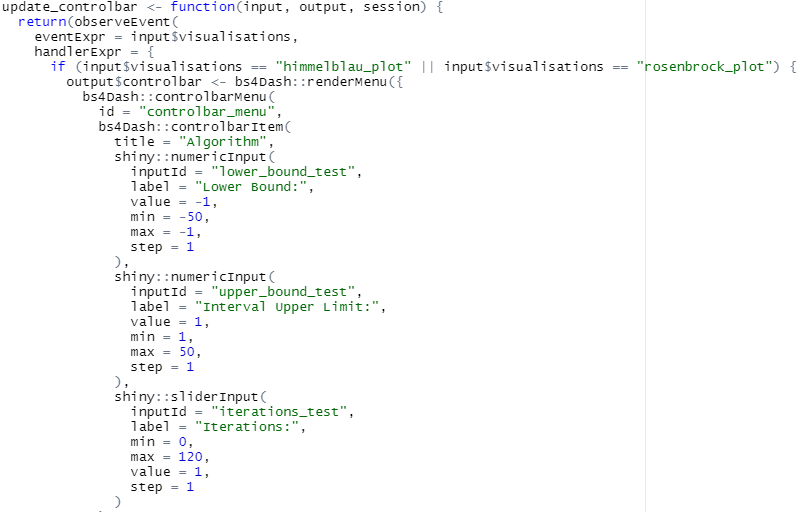
\includegraphics[scale=0.7]{"images/04_Visualisierung_des_Algorithmus/ui_slider_for_rose_him_plots_1.png"}
 \caption{Quellcode in fct\_update\_controlbar.R zur Darstellung interaktiver Elemente zur Festlegung des Such-Intervalls sowie der Anzahl an Iterationen zur Berechnung des Minimums mittels ACO}
 \label{fig:ui_RoseHimPlot_1}
\end{figure}

Um die Minima der Optimierungsfunktionen mittels ACO berechnen zu können, wird eine Funktion erstellt, welche in Abbildung \ref{fig:evoper_Minima_RoseHim_ACO} dargestellt wird. Hierbei wird das R-Package Evoper verwendet, das eine Implementierung des Ameisenalgorithmus beinhaltet. Die errechneten Minima werden neben den tatsächlichen Minima in einer zweiten Tabelle dargestellt und können so gut verglichen werden.
Sobald der Benutzer die Intervallgrenzen des Suchbereichs oder die Anzahl der Iterationen mithilfe der Schieberegler verändert, wird ein neues Ergebnis berechnet und die Tabelle der errechneten Minima wird aktualisiert. 
Je höher die Anzahl der Iterationen und je kleiner der Suchbereich, umso näher liegt das Ergebnis bei dem tatsächlichen Minimum bzw. an einem der tatsächlichen Minima. 
\newline
Bei der Himmelblaufunktion fällt auf, dass der Algorithmus bei Veränderung der Parameter maximal zwei der Minima findet. Unter welchen Voraussetzungen der Algorithmus in welches der Minima konvergiert, kann nicht festgelegt werden. Dies betont die Zuordnung des Ameisenalgorithmus zu den heuristischen Optimierungsverfahren, bei welchen unterschiedliche Start-Bedingungen zu unterschiedlichen Lösungen führen können. 

\begin{figure}[H]
 \centering
 \includegraphics[scale=0.7]{"images/04_Visualisierung_des_Algorithmus/evoper_calculate_Minimum_HimRose"}
 \caption{Quellcode in fct\_aco\_evoper.R um Minima der Rosenbrock- und Himmelblaufunktion mithilfe des ACO zu berechnen}
 \label{fig:evoper_Minima_RoseHim_ACO}
\end{figure}

 Den Quellcode der server-Funktion für die Generierung des dreidimensionalen Graphen der Rosenbrock-Funktion und der Tabellen für die tatsächlichen sowie mittels ACO errechneten Minima zeigt Abbildung \ref{fig:server_Minima_Rose_ACO}.

\begin{figure}[H]
 \centering
 \includegraphics[scale=.7]{"images/04_Visualisierung_des_Algorithmus/server_minima_rosenbrock"}
 \caption{Quellcode in mod\_rosenbrock\_tab.R um Rosenbrockfunktion darzustellen und Minimum mit Ergebnis des ACO zu vergleichen}
 \label{fig:server_Minima_Rose_ACO}
\end{figure}

Außerdem wird in mod\_rosenbrock\_tab.R und mod\_himmelblau\_tab.R jeweils ein Button erstellt, bei dessen Klick ein Popup erscheint, das die mathematische Formel der Rosenbrock bzw. der Himmelblau-Funktion darstellt. Wie dies in dem Tabreiter, der die Rosenbrock-Funktion darstellt, umgesetzt wird, zeigt Abbildung \ref{fig:server_mod_rosenbrock_tab_actionbutton}.

\begin{figure}[H]
 \centering
 \includegraphics{"images/04_Visualisierung_des_Algorithmus/server_mod_rosenbrock_tab_actionbutton"}
 \caption{Quellcode in mod\_rosenbrock\_tab.R um die Formel der Rosenbrock-Funktion in einem Popup darzustellen}
 \label{fig:server_mod_rosenbrock_tab_actionbutton}
\end{figure}

Mithilfe eines weiteren Info-Buttons in dem Navigations-Tab-Reiter, in welchem die Rosenbrock-Funktion visualisiert und optimiert wird, wird die Differenz des tatsächlichen Minimums zu dem mittels ACO berechneten Minimum dargestellt. Dies bewirkt, dass der Betrachter auf einen Blick die Qualität des berechneten Ergebnisses erkennt und die Verbesserung des Ergebnisses mit steigender Anzahl an Iterationen einfacher feststellen kann.  

Der dritte Tab-Reiter zur Visualisierung des Algorithmus hat das Ziel, dem Benutzer die iterative Näherung zum Minimum und die Zusammensetzung der errechneten Lösung aus den einzelnen Lösungen der Ameisen näher zu bringen. Hierfür wird die Himmelblau-Funktion als zu optimierende Funktion festgelegt. Interaktive Elemente ermöglichen es dem Benutzer erneut, den Suchbereich und die Anzahl an Iterationen, die der Algorithmus vornimmt, festzulegen. Zudem kann der Benutzer an dieser Stelle die Anzahl an Ameisen einer Generation festlegen. 
Das Minimum wird in diesem Fall nicht mithilfe des R-Pakets Evoper berechnet, sondern auf Basis der Implementierung von Garrigues \citep{Garrigues2019}, die in der Datei fct\_aco.R zu finden ist. Seine Funktionen werden in selbst erstellten Funktionen, die im Folgenden erläutert werden, aufgerufen und verwendet. 
Abbildung \ref{fig:makeStartGen} zeigt eine Deklaration der Funktionen, die initiale Ameisenwerte zufällig generieren unter Berücksichtigung der Anzahl der Ameisen sowie des Suchintervalls, das vom Benutzer festgelegt wurde.
In einer weiteren Funktion wird der eigentliche Iterationsschritt des Algorithmus durchgeführt und die neuen Positionen der Ameisen berechnet d.h. die neue Generation erstellt. Dies wird in Grafik \ref{fig:util_makeNewGen} abgebildet.


\begin{figure}[H]
 \centering
 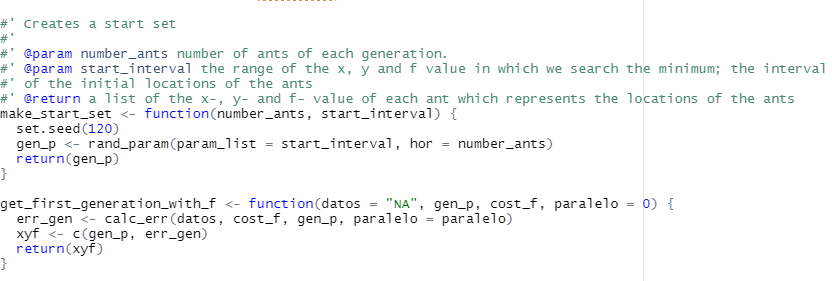
\includegraphics[scale=.7]{"images/04_Visualisierung_des_Algorithmus/util_makeStartGen.png"}
 \caption{Definition von Funktionen in global\_utils.R um Ameisengeneration zu initialisieren und Iterationsschritt durchzuführen}
 \label{fig:makeStartGen}
\end{figure}

\begin{figure}[H]
 \centering
 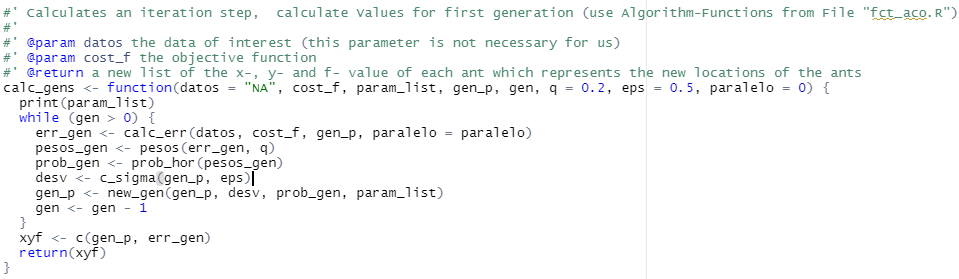
\includegraphics[scale=0.7]{"images/04_Visualisierung_des_Algorithmus/util_makeNewGen.png"}
 \caption{Definition von Funktionen in global\_utils.R um einen Iterationsschritt des ACO durchzuführen}
 \label{fig:util_makeNewGen}
\end{figure}

Um die Ameisenwerte, deren Mittelwert und die tatsächlichen Minima der Himmelblaufunktion graphisch darstellen zu können, werden die Werte in einer weiteren Funktion vorbereitet. Hierzu wird ein DataFrame erstellt, das neben den Spalten für die Koordinaten der Punkte eine zusätzliche Spalte besitzt, mithilfe welcher den Punkten eine Kategorie zugewiesen wird. Diese bestimmt, ob es sich bei dem Wert um einen Ameisenwert, einen Mittelwert oder ein tatsächliches Minimum handelt. Die Spalte wird benötigt, um den Punkten im Graphen je nach Kategorie unterschiedliche Farben verleihen zu können.
Die Deklaration dieser vorbereitenden Funktion zeigt Abbildung \ref{fig:util_prepareForPlot}.


\begin{figure}[H]
 \centering
 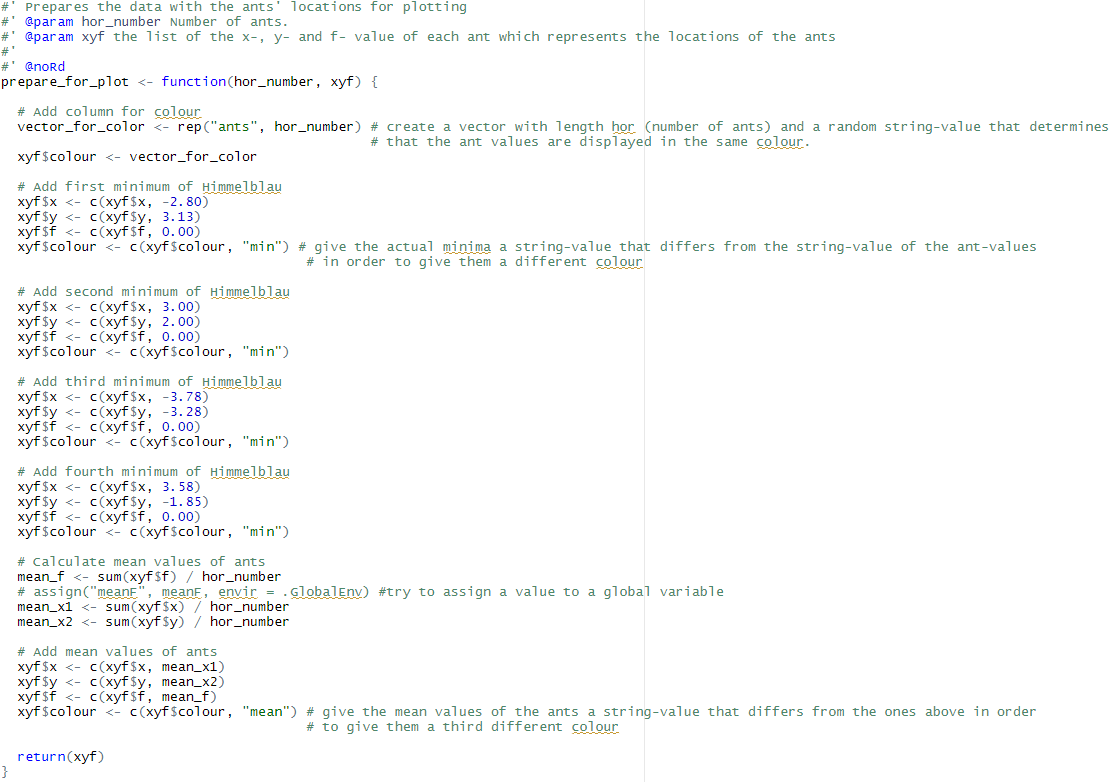
\includegraphics[scale=0.6]{"images/04_Visualisierung_des_Algorithmus/util_prepareForPlot.png"}
 \caption{Definition einer Funktionen in global\_utils.R um die Ameisenwerte, deren Mittelwert und die tatsächlichen Minima in einem Data Frame zu speichern, um sie in einem Graph darstellen zu können}
 \label{fig:util_prepareForPlot}
\end{figure}

Aufgerufen werden die genannten Funktionen in einem output-Element der \linebreak mod\_ant\_generations\_tab.R Datei (siehe Abbildung \ref{fig:antGenerations_plotGens}). Ebenfalls wird hier die Reaktivität der Parameter auf Benutzereingaben umgesetzt und der Graph dargestellt. 
Da das dreidimensionale Punktediagramm unter Verwendung des R-Pakets plotly erstellt wird, ist dessen Ansicht per Mausziehen verschiebbar und die Koordinaten eines Punkts werden angezeigt, sobald der Benutzer mit dem Mauszeiger darüber schwebt.
Dem Benutzer wird deutlich, dass sich der Algorithmus mit steigender Anzahl an Ameisen und Iterationen, einem der Minima nähert.  Wie vorhergehend erläutert, kann auch hier kein Kriterium identifiziert werden, das bestimmt, in welches der Minima der Algorithmus konvergiert.


\begin{figure}[H]
 \centering
 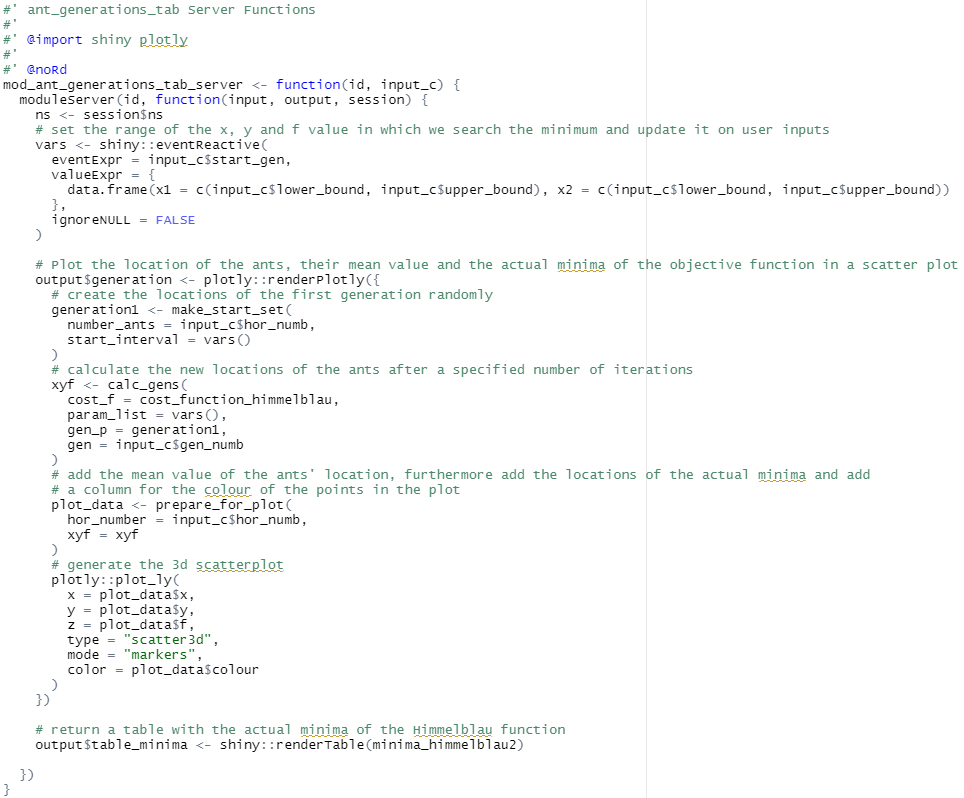
\includegraphics[scale=0.7]{"images/04_Visualisierung_des_Algorithmus/antGenerations_plotGens.png"}
 \caption{Server-Output Elemente der mod\_ant\_generations\_tab.R Datei um den Suchbereich zu aktualisieren, Ameisengenerationen zu berechnen und graphisch darzustellen}
 \label{fig:antGenerations_plotGens}
\end{figure}